\documentclass[border=3pt]{standalone}
% Preâmbulo compartilhado pelos diagramas TikZ da aula 9 de IHC (Princípios e Diretrizes)
\usepackage[T1]{fontenc}
\usepackage[utf8]{inputenc}
\usepackage{lmodern}
\usepackage{amsmath}
\usepackage{xcolor}
\usepackage{tikz}
\usetikzlibrary{arrows.meta,angles,quotes,decorations.pathmorphing,decorations.pathreplacing,calc,
                positioning,shapes.geometric,shapes.misc,backgrounds,fit,
                math}

% Paleta (mesma dos SVGs originais)
% Paleta da disciplina de IHC: acento roxo (#755099), da capa do livro.
% (o nome "dblue" é mantido para não alterar todos os diagramas)
\definecolor{dblue}{HTML}{755099}
\definecolor{dorange}{HTML}{B3541E}
\definecolor{dgreen}{HTML}{4A7C59}
\definecolor{dred}{HTML}{9C4B4B}
\definecolor{dcream}{HTML}{F4F1EA}
\definecolor{dshade}{HTML}{DDD7C9}

% Função gaussiana (não normalizada por padrão de escala visual)
\pgfmathdeclarefunction{gauss}{3}{%
  \pgfmathparse{1/(#3*sqrt(2*pi))*exp(-((#1-#2)^2)/(2*#3^2))}%
}

% Estilos comuns (prefixo d... para não colidir com chaves internas do pgf)
\tikzset{
  >={Stealth[length=2mm]},
  dguide/.style={gray!55, dashed, line width=0.4pt},
  daxis/.style={gray!60, line width=0.7pt, ->},
  dbody/.style={fill=black!3, draw=black!80, line width=1pt},
  dacc/.style={draw=dblue, line width=1pt},
  dlbl/.style={black!55, font=\small},
  dsub/.style={black!45, font=\footnotesize},
  dstate/.style={circle, draw=black!80, fill=dcream, line width=1pt,
                 minimum size=17mm, font=\large, inner sep=1pt},
  dobs/.style={circle, draw=black!80, fill=dshade, line width=1pt,
               minimum size=14mm, font=\large, inner sep=1pt},
  dbox/.style={rounded corners=2pt, draw=black!80, fill=dcream, line width=1pt,
               align=center, inner sep=6pt},
  dop/.style={circle, draw=black!80, fill=white, line width=1pt,
              minimum size=6mm, inner sep=0pt, font=\small},
  dtrans/.style={->, dblue, line width=1pt},
  dmeas/.style={->, dorange, line width=1pt},
  dcurve/.style={line width=1pt, dblue},
  dcurveb/.style={line width=1.4pt, dorange},
}

\begin{document}
\hyphenpenalty=10000 \exhyphenpenalty=10000 \tolerance=9999 \emergencystretch=3em
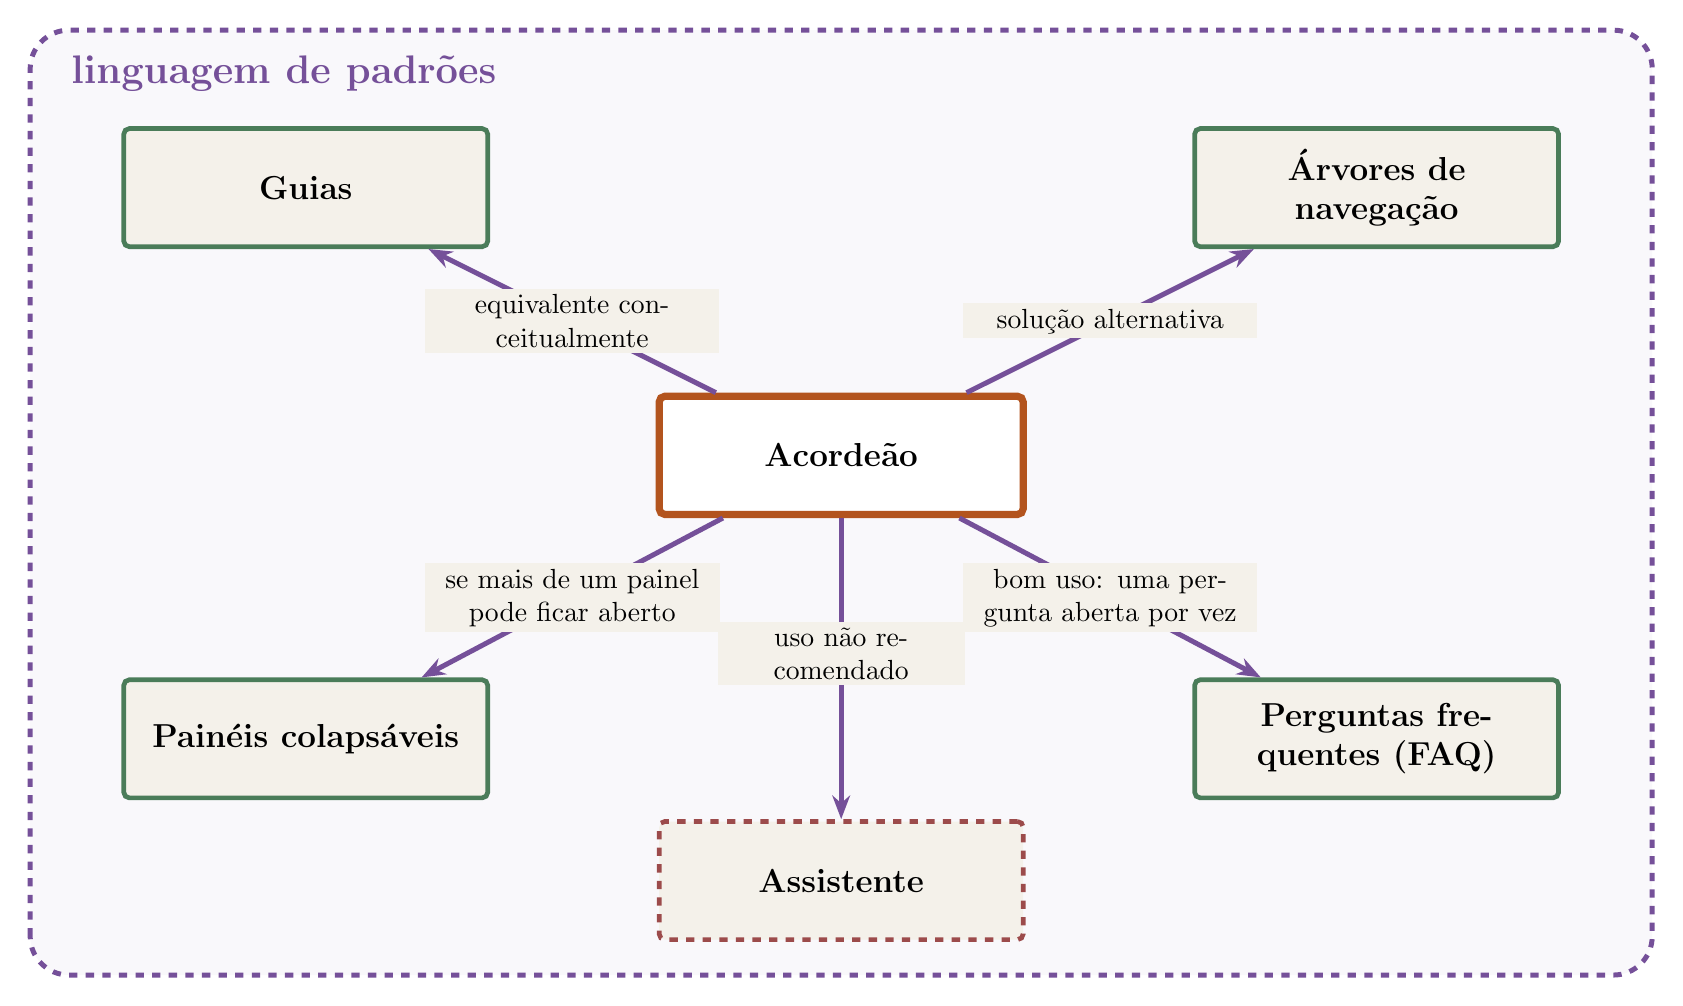
\begin{tikzpicture}[x=1cm,y=1cm]
\tikzset{n/.style={dbox, text width=4.2cm, minimum height=1.5cm, font=\large\bfseries, line width=1.7pt},
        e/.style={dtrans, line width=1.8pt, -{Stealth[length=3mm]}},
        l/.style={midway, fill=dcream, inner sep=2pt, font=\normalsize, text=black, text width=3.6cm, align=center}}
\draw[draw=dblue, dashed, line width=1.8pt, rounded corners=14pt, fill=dblue!4] (-0.6,-2.2) rectangle (20.0,9.8);
\node[font=\Large\bfseries, dblue, anchor=north west] at (-0.2,9.6) {linguagem de padrões};
\node[n, draw=dorange, line width=2.6pt, fill=white] (a) at (9.7,4.4) {Acordeão};
\node[n, draw=dgreen] (g) at (2.9,7.8) {Guias};
\node[n, draw=dgreen] (t) at (16.5,7.8) {Árvores de navegação};
\node[n, draw=dgreen] (p) at (2.9,0.8) {Painéis colapsáveis};
\node[n, draw=dgreen] (f) at (16.5,0.8) {Perguntas frequentes (FAQ)};
\node[n, draw=dred, dashed] (s) at (9.7,-1.0) {Assistente};
\draw[e] (a) -- (g) node[l] {equivalente conceitualmente};
\draw[e] (a) -- (t) node[l] {solução alternativa};
\draw[e] (a) -- (p) node[l] {se mais de um painel pode ficar aberto};
\draw[e] (a) -- (f) node[l] {bom uso: uma pergunta aberta por vez};
\draw[e] (a) -- (s) node[l, pos=0.45, text width=3.0cm] {uso não recomendado};
\end{tikzpicture}
\end{document}
